\section{Pre-amplifier}
In order to transfer as much of the signal from the guitar to the \gls{dsp} as possible, and avoid a significant voltage division between the guitar and the \gls{dsp}, a \gls{preamp} will be designed. The output impedance of the guitar is measured and the result is shown in \autoref{app:output_impedance}. This shows that the output impedance for a guitar is not the same from \SI{10}{\hertz} to \SI{22}{\kilo\hertz}. The output impedance is always more than \SI{6220}{\ohm} and the maximum output impedance is \SI{73.08}{\kilo\ohm}, for the measured guitar. Therefore the \gls{preamp} must have an input impedance, much higher than \SI{73.08}{\kilo\ohm}, to avoid a significant voltage division in the frequency area from \SI{10}{\kilo\hertz} to \SI{22}{\kilo\hertz}. 

\subsection{The operational-amplifier}

In \autoref{app:guitar_max_amplitude} it is seen that the maximum output signal from the guitar is about $\SI{1}{\volt}_{peak}$. The 
\gls{dsp} have a typical input signal level of $\SI{0.5}{\volt}_{RMS}$ which give a peak value of $\SI{0.707}{\volt}_{peak}$ \citep{TLV320AIC3204}. To make a general \gls{preamp} that works with more guitar than only the measured guitar, the \gls{preamp} will be designed with a volume control. It is chosen that the \gls{preamp} shall have a voltage gain of approximate \SI{3}{\decibel} and the input impedance shall be more than ten times the guitar output impedance. The \gls{preamp} will be designed to fit into a \SI{6.33}{\milli\meter}  jack connector house, and therefore the chosen \gls{opamp} is the ST ts424 \citep{TS464} and the \gls{preamp} will be designed to fit this \gls{opamp}. 
	An \gls{opamp} often have an input impedance of more than \SI{1}{\mega\ohm} and have a gain of about \SI{100}{\decibel}, and after the feedback circuit is implemented on the \gls{opamp} the input impedance is even higher and the output impedance is even lower. A simple diagram of the overall \gls{preamp}, which will be designed, is shown in \autoref{fig:simple_preamp}. 

\begin{figure}[h!]
\centering
\begin{circuitikz}\draw (0,0)
(0,0)to[short, o-]node[left,above]{$Input$}(1,0)
to[amp, t=$G1$]  (3,0)
to[short] (3,0)
to[pR=$ $](3,-2)
to[short](3,-2)node[ground]{}(3.5,-1)
to[short] (4,-1)
to[short] (4,0)
to[amp, t=$G2$]  (6,0)
(6,0)to[short, -o]node[left,above]{$Output$}(7,0)
%to[short] (0,0)
;\end{circuitikz}
\caption{A simple block diagram of the overall \gls{preamp}.}
\label{fig:simple_preamp}
\end{figure}


\subsection{Design of $G1$ resistor}
The first amplification in the \gls{opamp}, $G1$ in \autoref{fig:simple_preamp}, can ether be working in a non inverting or an inverting \gls{opamp} configuration. Since the \gls{preamp} shall have a gain of \SI{6}{\decibel} and a high input impedance, the non inverting \gls{opamp} configuration will be used, because it is a voltage-seriel feedback configuration. The seriel feedback configuration gives a higher input impedance than a parallel feedback, because the feedback circuit is in series with the input imperdance of the \gls{opamp} and not i parallel. The schematics of a non inverting \gls{opamp} is shown in \autoref{fig:preamp_opamp}.

\begin{figure}[h!]
\centering
\begin{circuitikz}\draw (0,0)
node[op amp,yscale=-1] (opamp) {} 
(-3,-3.5)
to[R=$R_{Bias}$] (-3,0.5)
to[short](opamp.+) 
(-5,0.5)to[short, o-]node[left,above]{$Input$} (-3,0.5)
(opamp.-) 
(opamp.out) 
to[short] (2,0)
to[short] (2,-1.5)
to[R=$R_F$] (-1.5,-1.5)
to[short] (-1.5,-0.5)
to[short] (-1,-0.5)
(-1.5,-1.5)to[R=$R_1$] (-1.5,-3.5)
(2,-1.5)to[pR, l_=$R_V$] (2,-3.5)
(2.5,-2.5)to[short, -o]node[left,above]{$Output$} (4,-2.5)
(-3,-3.5)to[short](2,-3.5)
(-1.5,-3.5)to[V=$V_{Offset}$] (-1.5,-5)node[ground]{}(-1.5,-5.5)
;\end{circuitikz}
\caption{The schematic of $G1$, see \autoref{fig:simple_preamp}.}
\label{fig:preamp_opamp}
\end{figure}

The output of $G1$ is looking into $G2$ which is a \gls{opamp} with an input impedance higher than \SI{1}{\mega\ohm}, and therefor the calculations can be made without taking $G2$ into account. The calculation is also without the $V_{Offset}$ power supply, because a voltage power supply is a short circuit with respect to impedances.  The equivalent schematic of a non inverting \gls{opamp} is as follows in  \autoref{fig:preamp_opamp_equa}.

\begin{figure}[h!]
\centering
\begin{circuitikz}\draw (0,0)
to[R=$R_{Bias}$] (0,-2)node[ground]{}(0,-2.5)
(0,0)to[R=$Z_{i}$] (2,0)
to[R=$Z_{i\beta}$] (4,0)
to[V=$\beta \cdot V_o$] (4,-2)node[ground]{}(4,-2.5)
(0,0)to[short, -o]node[left,above]{$Z_{Input}$} (-3,0)
;\end{circuitikz}
\caption{The equivalent input impedance schematic of $G1$, see \autoref{fig:simple_preamp}.}
\label{fig:preamp_opamp_equa}
\end{figure}

\newpage

The calculation of $Z_{i\beta}$ is done using \autoref{eq:preamp_ib}

\begin{equation}\label{eq:preamp_ib}
        Z_{i\beta} = R_F\parallel R_1
        \addunit{\si{\ohm}}
    \end{equation}

    \startexplain
        \explain{$R_1$ is a resistor in the feedback circuit}{\si{\ohm}}
        \explain{$R_F$ is a resistor in the feedback circuit}{\si{\ohm}}
        \explain{$Z_{i\beta}$ the impedance of the feedback circuit}{\si{\ohm}}
    \stopexplain

Calculating of $\beta$ is done by following \autoref{eq:preamp_beta}

\begin{equation}\label{eq:preamp_beta}
        \beta = \frac{R_1}{R_1 + R_F}
        \addunit{\si{1}}
    \end{equation}
    \startexplain
        \explain{$\beta$ is the feedback factor}{\si{1}}
    \stopexplain


The resulting input impedance of the \gls{preamp} will be as following \autoref{eq:preamp_result}.

\begin{equation}\label{eq:preamp_result}
        Z_{In_{G1}} = R_{Bias}\parallel ((Z_i + Z_{i \beta}) \cdot (1+\beta \cdot A)) \simeq R_{Bias}
        \addunit{\si{\ohm}}
    \end{equation}

    \startexplain
        \explain{$Z_{In_{G1}} $ is the resulting input impedance of $G1$}{\si{\ohm}}
        \explain{$R_{Bias}$ An bias resistor}{\si{\ohm}}
        \explain{$Z_i$ The input impedance of the \gls{opamp}}{\si{\ohm}}
         \explain{$A$ is the gain of the \gls{opamp}}{\si{1}}
    \stopexplain

$R_{Bias}$ is chosen to \SI{1}{\mega\ohm}.
The feedback circuit will increase the $(Z_{i}+Z_{i\beta})$ by a factor of $(1+\beta \cdot A')$, and since the input impedance of an \gls{opamp} is over \SI{1}{\mega\ohm}, the feedback resistor values dose not matter, besides their relation. The feedback circuit will also decrease the output impedance by a factor of $(1+\beta \cdot A)$, which also entails that only the relation between the feedback resistors is important. The circuit in \autoref{fig:preamp_opamp_equa_out} shows the output impedance equivalent circuit of the \gls{opamp}.

\begin{figure}[h!]
\centering
\begin{circuitikz}\draw (0,0)
to[V=$A \cdot V_i$] (0,-3)
(0,0)to[R=$Z_o$](2,0)
to[R=$Z_{o\beta}$](2,-3)
(2,0)to[short](4,0)
(4,0)to[pR, l_=$R_V$](4,-3)
(0,-3)to[short, -o](6,-3)
(4.5,-1.5)to[short, -o](6,-1.5)
;\end{circuitikz}
\caption{The equivalent output impedance schematic of $G1$, see \autoref{fig:simple_preamp}}
\label{fig:preamp_opamp_equa_out}
\end{figure}


Calculating of $Z_{o\beta}$ is done by following \autoref{eq:preamp_beta_out}

\begin{equation}\label{eq:preamp_beta_out}
        Z_{o\beta} = R_F+R_1
        \addunit{\si{\ohm}}
    \end{equation}

A voltage power supply is a short cut with respect to impedance, so the resulting output impedance of $G1$ is calculated by following \autoref{eq:preamp_zout_out} 

\begin{equation}\label{eq:preamp_zout_out}
        Z_{out_{G1}} = \frac{ Z_{o\beta} \parallel Z_{o} }{1+\beta \cdot A'}
        \addunit{\si{\ohm}}
    \end{equation}
    \startexplain
        \explain{$A' =A \cdot \frac{Z_{o\beta}}{Z_o+Z_{o\beta}} \cdot \frac{Z_i}{Z_i+Z_{i\beta}}$ }{\si{1}}
\explain{$Z_{out_{G1}}$ is the total output impedance of $G1$ }{\si{\ohm}}
    \stopexplain

$R_V$ is chosen to \SI{10}{\kilo\ohm} to make as small a voltage division between $Z_{out}$ and $R_V$ as possible. In another way, to keep the voltage over $Z_{out_{G1}}$ as small as possible. The $R_F$ is chosen to be \SI{5}{\kilo\ohm} \todo[inline]{Input and output impedance MUST be measured}


The approximated amplification of a non inverting \gls{opamp} is given by \autoref{eq:preamp_amplification}

\begin{equation}\label{eq:preamp_amplification}
        G =1+\frac{R_F}{R_1}
        \addunit{\si{1}}
    \end{equation}

    \startexplain
        \explain{$G$ is the amplification of $G1$}{\si{1}}
    \stopexplain

Since the tested guitar have en amplitude of \SI{1}{\volt} it is chosen that the \gls{preamp} only shall be able to amplify by a factor of 2. Then  $R_1$ is founded to be \SI{5}{\kilo\ohm} by isolate $R_1$ in the above \autoref{eq:preamp_amplification}.
 
   
\subsection{Design of $G1$ DC offset}
The \gls{preamp} will be powered by one positive power supply of \SI{5}{\volt} and therefore a DC offset must be implemented to make the signal be swing around \SI{2.5}{\volt}. 
The design of the voltage offset power supply will be done by two resistors which divide the voltage by two equals, and afterwards an \gls{opamp} is used as buffer  to make a small output impedance. Because the \gls{opamp} have a impedance of more than \SI{1}{\mega\ohm} the resistor size does not matter, but a non ideal \gls{opamp} do have a bias current in the input, that will affect the division if the resistors are to large. To keep the division approximate to two, the resistors shall be at least ten times smaller than the input impedance of the \gls{opamp}. The voltage offset power supply circuit is designed as in \autoref{fig:preamp_voffset}.
    
  \begin{figure}[h!]
\centering
\begin{circuitikz}\draw (0,0)
node[op amp,yscale=-1] (opamp) {} 
(-9,0.5)to[short, o-]node[right,above]{$V_s$} (-8,0.5)
to[R=$R_{2}$]
(-5,0.5)to[C=$C_{Offset}$](-5,-2)node[ground]{}
(-5,0.5)to[short]
(-3,0.5)to[R=$R_{Offset}$](-3,-2)node[ground]{}
(opamp.+) 
(-3,0.5)to(opamp.+) 
(opamp.out) 
to[short] (2,0)
to[short] (2,-1.5)
to[short] (-1.5,-1.5)
to[short] (-1.5,-0.5)
to[short] (-1,-0.5)
(2,0)to[short, -o] (4,-0)node[left,above]{$V_{Offset}$}
;\end{circuitikz}
\caption{The offset power supply to $G1$, see \autoref{fig:preamp_opamp} }
\label{fig:preamp_voffset}
\end{figure}
  
Where $C_{Offset}$ is used to stabilize the voltage at the input of the \gls{opamp} and the calculation of $R_{Offset}$ and $R_{2}$ is done as in \autoref{eq:preamp_offset}.

\begin{equation}\label{eq:preamp_offset}
        R_{Offset} = R_{2} = \frac{Z_{in}}{10}
        \addunit{\si{\ohm}}
    \end{equation}

    \startexplain
        \explain{$Z_{in}$ is the input impedance of the \gls{opamp}}{\si{\ohm}}
        \explain{$R_2$ is the upper resistor in the voltage division circuit}{\si{\ohm}}
        \explain{$R_{offset}$ is the lower resistor in the voltage division circuit}{\si{\ohm}}
    \stopexplain
    
\subsection{Design of input and output DC blocking}

The total circuit of the \gls{preamp} is as in \autoref{fig:preamp_total}, where the \gls{opamp} to the far right without any resistors in the feedback loop, is $G2$.
%and the design of $G1$ input capacitor $C_{In}$ and  $G2$ output capacitor $C_{Out}$ will be done beneath the full circuit \autoref{fig:preamp_total}.

\begin{figure}[h!]
\centering
\begin{circuitikz}\draw 
(-5,0.5) node[anchor=south] {$S_{In}$}
(-5,-5.5) node[anchor=south] {$V_{in}$}
(8.5,-3) node[anchor=south] {$S_{Out}$}
(0,0)node[op amp,yscale=-1] (opamp1) {} 
(-3,-3.5)
to[R=$R_{Bias}$] (-3,0.5)
to[short](opamp1.+) 
(-5,0.5)to[C=$C_{In}$, o-] (-3,0.5)
(opamp1.-) 
(opamp1.out) 
to[short] (2,0)
to[short] (2,-1.5)
to[R=$R_F$] (-1.5,-1.5)
to[short] (-1.5,-0.5)
to[short] (-1,-0.5)
(-1.5,-1.5)to[R=$R_1$] (-1.5,-3.5)
(2,-1.5)to[pR, l_=$R_V$] (2,-3.5)
(2.5,-2.5)to[short](4,-2.5)
(-3,-3.5)to[short](2,-3.5)
(5,-3) node[op amp,yscale=-1] (opamp2) {} 
(opamp2.-) 
(opamp2.+) 
(opamp2.out) 
to[short] (7,-3)
to[short] (7,-4.5)
to[short] (3.5,-4.5)
to[short] (3.5,-3.5)
to[short] (4,-3.5)
(7,-3)to[C=$C_{Out}$, -o](8.5,-3)
(2,-6)node[op amp,yscale=-1] (opamp3) {} 
(-5,-5.5)to[R=$R_{2}$, o-]
(-3,-5.5)to[C=$C_{Offset}$](-3,-7.5)node[ground]{}
(-3,-5.5)to[short]
(-1,-5.5)to[R=$R_{Offset}$](-1,-7.5)node[ground]{}
(opamp3.+) 
(-1,-5.5)to(opamp3.+) 
(opamp3.out) 
to[short] (4,-6)
to[short] (4,-7.5)
to[short] (0.5,-7.5)
to[short] (0.5,-6.5)
to[short] (1,-6.5)
(4,-6) to[short] (4,-5)
to[short] (2,-5)
to[short] (2,-3.5)
;\end{circuitikz}
\caption{The full schematic of the \gls{preamp}, $G1$ and $G2$, see \autoref{fig:simple_preamp}}
\label{fig:preamp_total}
\end{figure}

$C_{In}$ will be designed to have a cut-off frequency a decade beneath the audibility area. This result in a cut-off frequency of \SI{2}{\hertz}. The calculation of $C_{In}$ is done by following \autoref{eq:preamp_cin}.

    
\begin{subequations}\label{eq:preamp_cin}
\begin{equation}
        C_{In} \geq  \frac{1}{2 \pi \cdot Z_{In_{G1}} \cdot f}
        \addunit{\si{\farad}}
    \end{equation}
\centering
$\Updownarrow$
\begin{equation}
        \SI{80}{\nano\farad} \geq  \frac{1}{2 \pi \cdot 1M\ohm \cdot 2Hz}
        \addunit{\si{\farad}}
    \end{equation}
 \end{subequations}    
    

    \startexplain
         \explain{$C_{In}$ is the input capacitor}{\si{\farad}}
        \explain{$Z_{In}$ is the input impedance of $G1$}{\si{\ohm}}
        \explain{$f$ is the cut-off frequency}{\si{\hertz}}
    \stopexplain
    
$C_{Out}$ will be designed to have a cut-off frequency at a decade over the audibility area, which will result in a cross frequency of \SI{200}{\kilo\hertz}. The calculation of $C_{Out}$ is done by following \autoref{eq:preamp_cout}.


\begin{subequations}\label{eq:preamp_cout}
\begin{equation}
        C_{In} \geq  \frac{1}{2 \pi \cdot Z_{In,\gls{dsp}} \cdot f}
        \addunit{\si{\farad}}
    \end{equation}
\centering
$\Updownarrow$
\begin{equation}
         \SI{400}{\pico\farad} \geq  \frac{1}{2 \pi \cdot 20k\ohm \cdot 20kHz}
        \addunit{\si{\farad}}
    \end{equation}
 \end{subequations}    

    \startexplain
     \explain{$C_{Out}$ is the output capacitor}{\si{\farad}}
        \explain{$Z_{In,\gls{dsp}}$ is the input impedance of the \gls{dsp}}{\si{\ohm}}
 \explain{$f$ is the cut-off frequency}{\si{\hertz}}
    \stopexplain
    
The $C_{Offset}$ is selected to be separated into one \SI{100}{\nano\farad}- and one \SI{1}{\micro\farad}- capacitor, and both $C_{In}$ and $C_{Out}$ is chosen to be  \SI{10}{\micro\farad} 
 
\subsection{\gls{pcb} layout} 
The signal cable will have a capacitive effect on the signal, from the guitar to the \gls{preamp}, and this will cause a low pass filter. In order to avoid the low pass problem with the cable, the \gls{preamp} will be designed to fit inside a \SI{6.35}{\milli\meter} Jack connector house. This requires that the \gls{pcb} has a maximum size of  \SI{1}{\centi\meter} times \SI{2.5}{\centi\meter}. The used cable from the \gls{dsp} to the \gls{preamp} is a balanced cable, where the shield is used as ground to both signal and power. The red wire is used as signal wire and the black wire is used as positive power wire. The resulting \gls{preamp} layout is as in \autoref{fig:preamp_layout}.
 
 \begin{figure}[h]
	\centering
		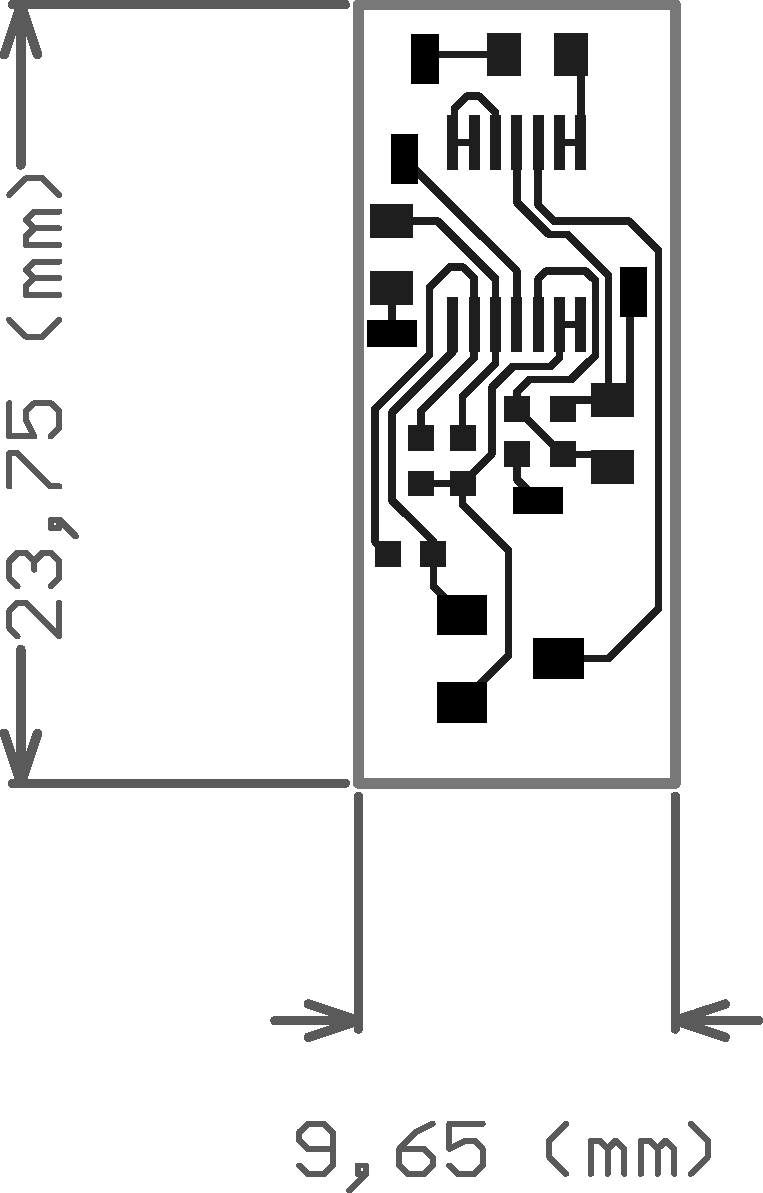
\includegraphics[width=0.2\textwidth]{PreAmp.pdf}
		\caption{The \gls{preamp} layout}
		\label{fig:preamp_layout}
\end{figure}

In \autoref{app:opamp_impedance} it is measured that $Z_i =$\SI{9.18}{\mega\ohm} which follows the assumption, but $Z_o$ is measured to \SI{9.06}{\kilo\ohm} which means that $R_V$ might have to be changed. 
 